\documentclass[12pt,a4paper]{article}

% Useful packages
\usepackage[utf8]{inputenc}
\usepackage[T1]{fontenc}
\usepackage[english]{babel}
\usepackage{amsmath,amsfonts,amssymb}
\usepackage{graphicx} % Package to include images
\usepackage{hyperref}
\usepackage{enumitem}
\usepackage{geometry}
\geometry{margin=2.5cm}

% Title
\title{Project Opeationalizing Machine Learning on SageMaker}
\author{Geraldo Margjini}
\date{\today}

\begin{document}

\maketitle

\begin{abstract}
This document presents the write-up of the project, including answers and explanations to the assigned questions.
\end{abstract}

\tableofcontents
\newpage

\section{Step 1: Training and Deployment on Sagemaker}
\subsection{Initial Steps}
I selected an ml.t3.medium instance because the dataset I’m working with is small. This instance type is among the most cost-effective options and is sufficient for the task at hand. Moreover, it falls within my AWS Free Tier usage.
\begin{figure}[htbp]
  \centering
  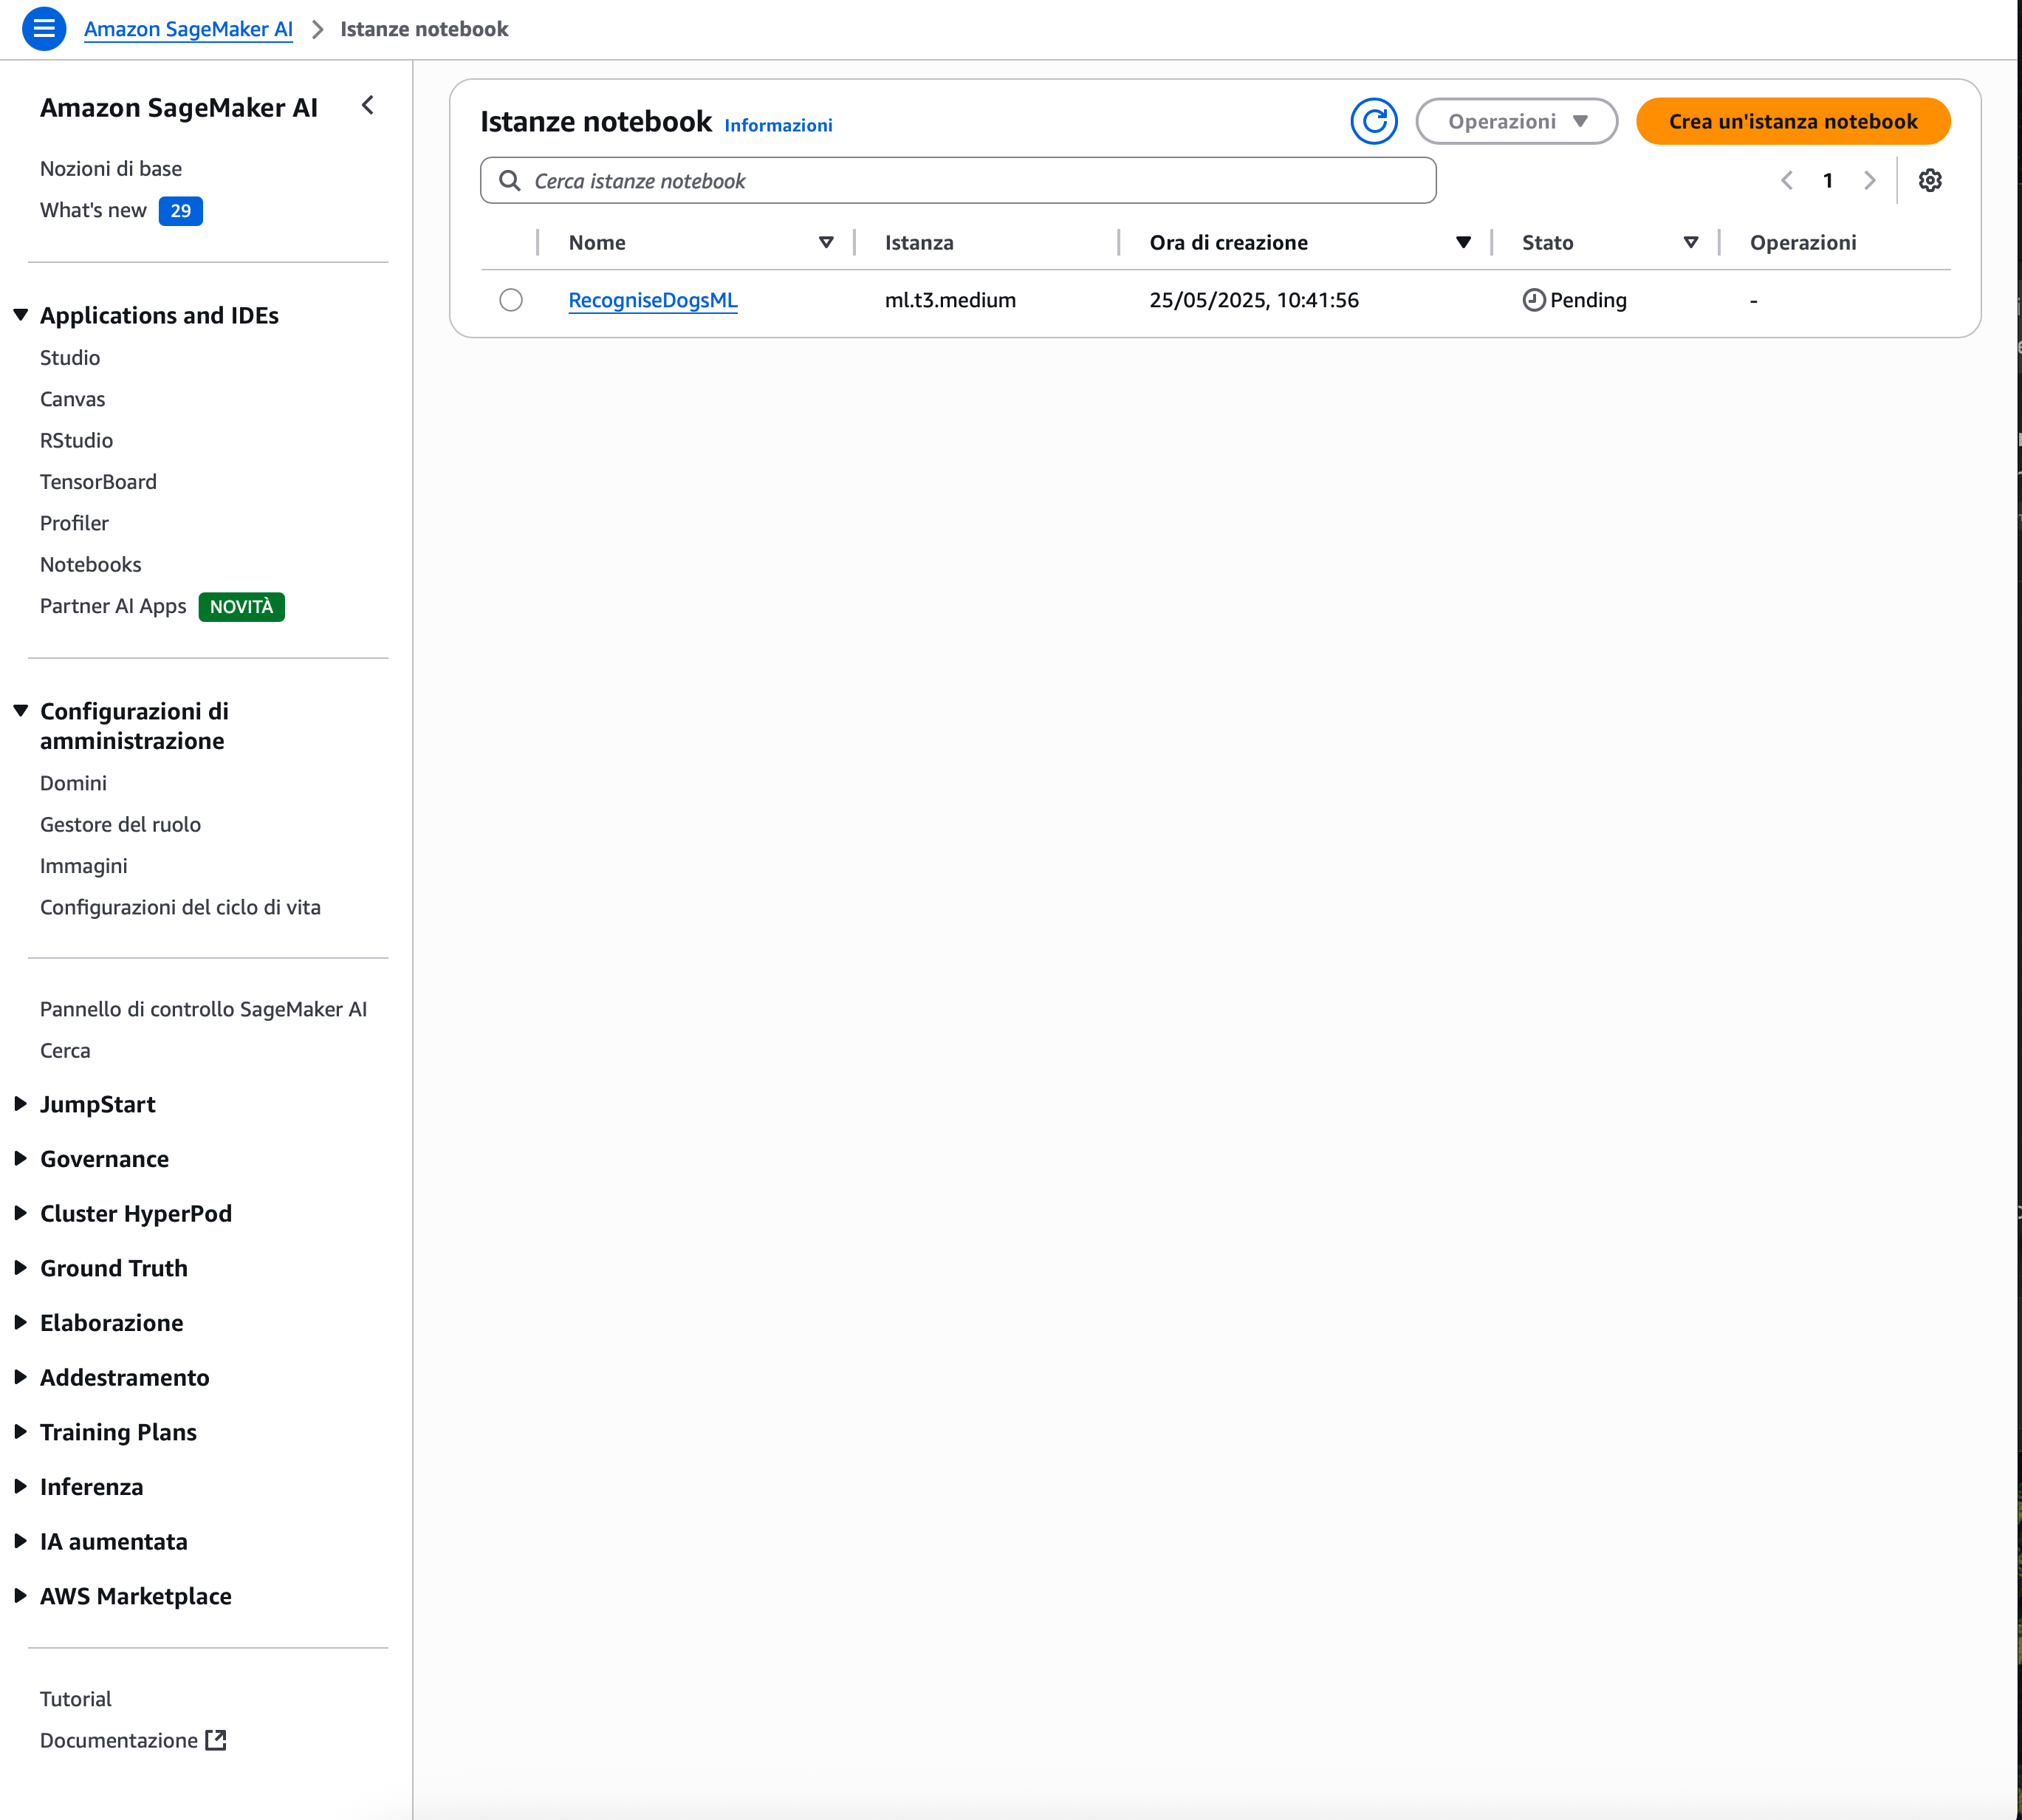
\includegraphics[width=0.5\textwidth]{img/Screenshot 2025-05-25 alle 10.43.02.png}
  \caption{screenshot showing a created notebook instance on Sagemaker.}
  \label{fig:example}
\end{figure}
\subsection{Download the data in the S3 Bucket}
So the next step is to create a new S3 Bucket that i called \textit{reco-dogs} and run the three first cell to download the data of different dog breads ( 133 dog breads, 6680 training, 835 validation and 836 test images).
\begin{figure}[htbp]
  \centering
  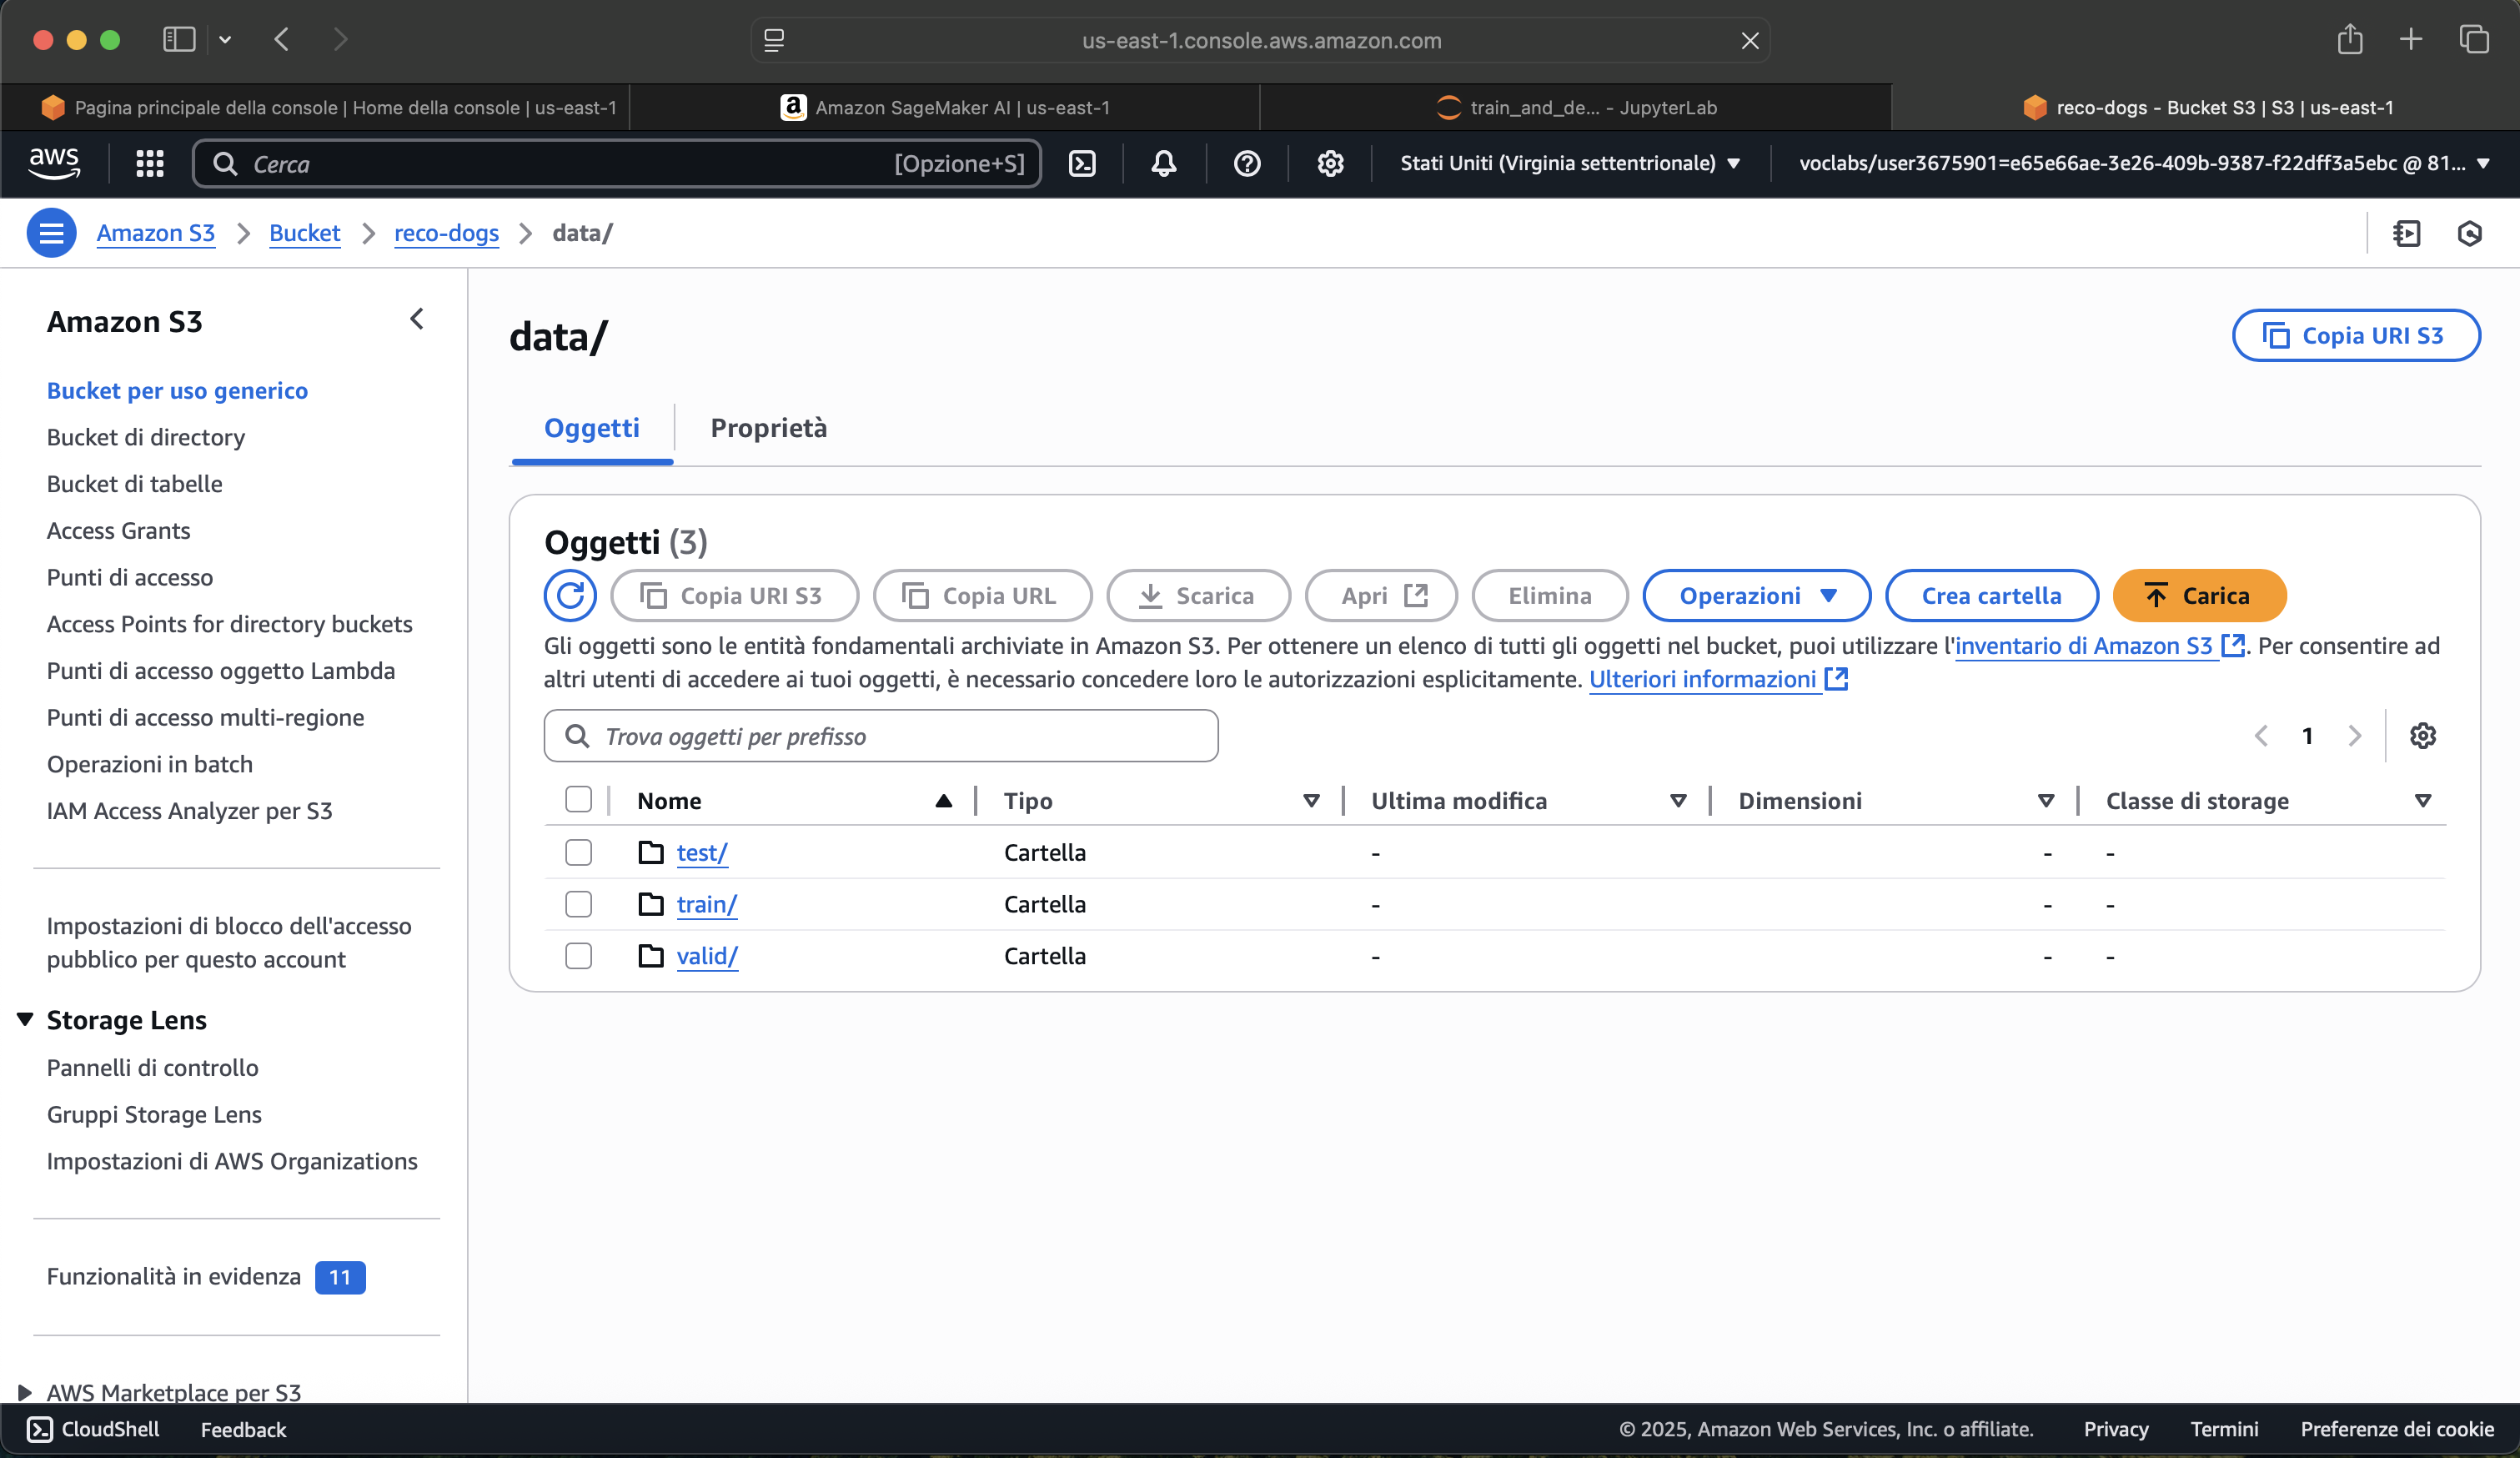
\includegraphics[width=0.7\textwidth]{img/Screenshot 2025-06-07 alle 17.03.13.png}
  \caption{screenshot showing a created and downloaded the Data in my S3 Bucket.}
  \label{fig:example}
\end{figure}
\subsection{Single Instance Training: Training and Deployment}
I created a tuning job with the following parameter and got \begin{verbatim}{'batch_size': 256, 'learning_rate': '0.002896533293199136'} \end{verbatim} as best hyperparameters.
\begin{verbatim}
tuner = HyperparameterTuner(
    estimator,
    objective_metric_name,
    hyperparameter_ranges,
    metric_definitions,
    max_jobs=2,
    max_parallel_jobs=1,  # you once have one ml.g4dn.xlarge instance available
    objective_type=objective_type
)
\end{verbatim}
So then i trained using this parameter with a ml.m5.xlarge:
\begin{verbatim}
estimator = PyTorch(
    entry_point='hpo.py',
    base_job_name='dog-pytorch',
    role=role,
    instance_count=1,
    instance_type='ml.m5.xlarge',
    framework_version='1.4.0',
    py_version='py3',
    hyperparameters=hyperparameters,
    ## Debugger and Profiler parameters
    rules = rules,
    debugger_hook_config=hook_config,
    profiler_config=profiler_config,
)
\end{verbatim}

So following we have the screenshot of the Endpoint created:

\begin{figure}[htbp]
  \centering
  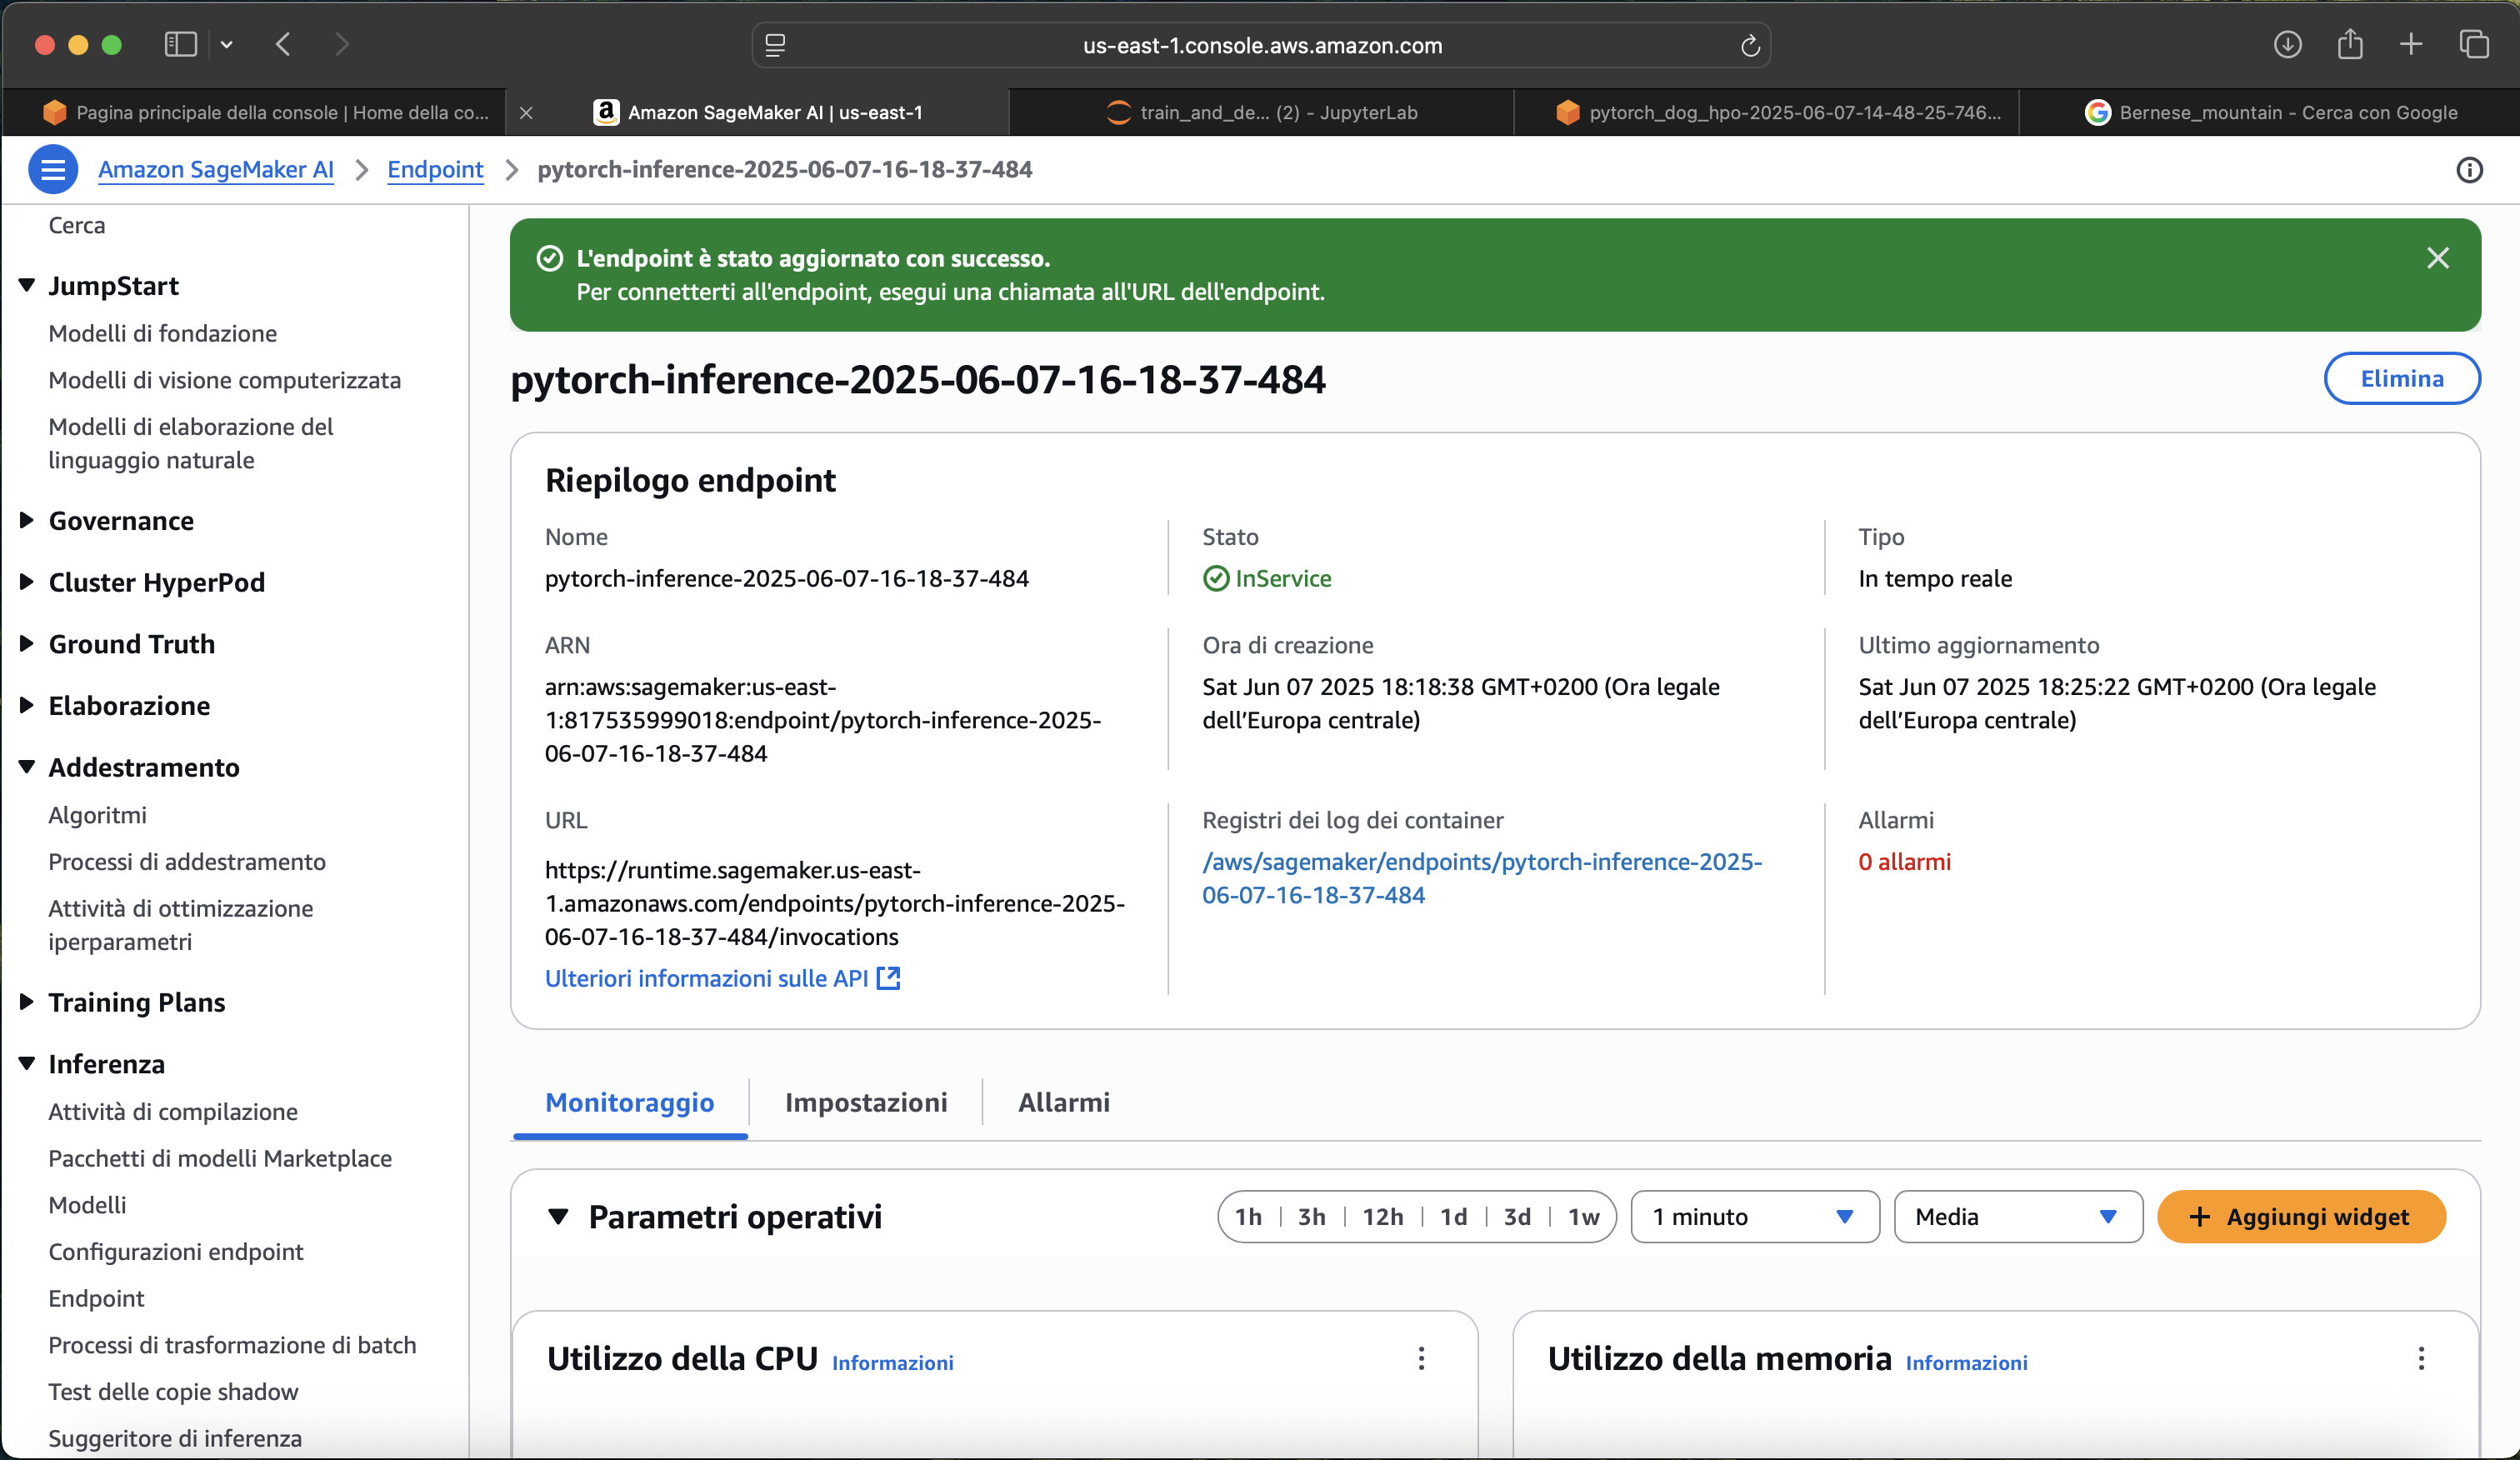
\includegraphics[width=0.7\textwidth]{img/Screenshot 2025-06-07 alle 18.34.17.png}
  \caption{screenshot showing a created Endpoint for the single instance.}
  \label{fig:example}
\end{figure}

\subsection{Multy Instance Training: Training and Deployment}
For the Multy instance i used the value for the \begin{verbatim}instance_count=4\end{verbatim} to train four instances at time.

\newpage

\begin{figure}[htbp]
  \centering
  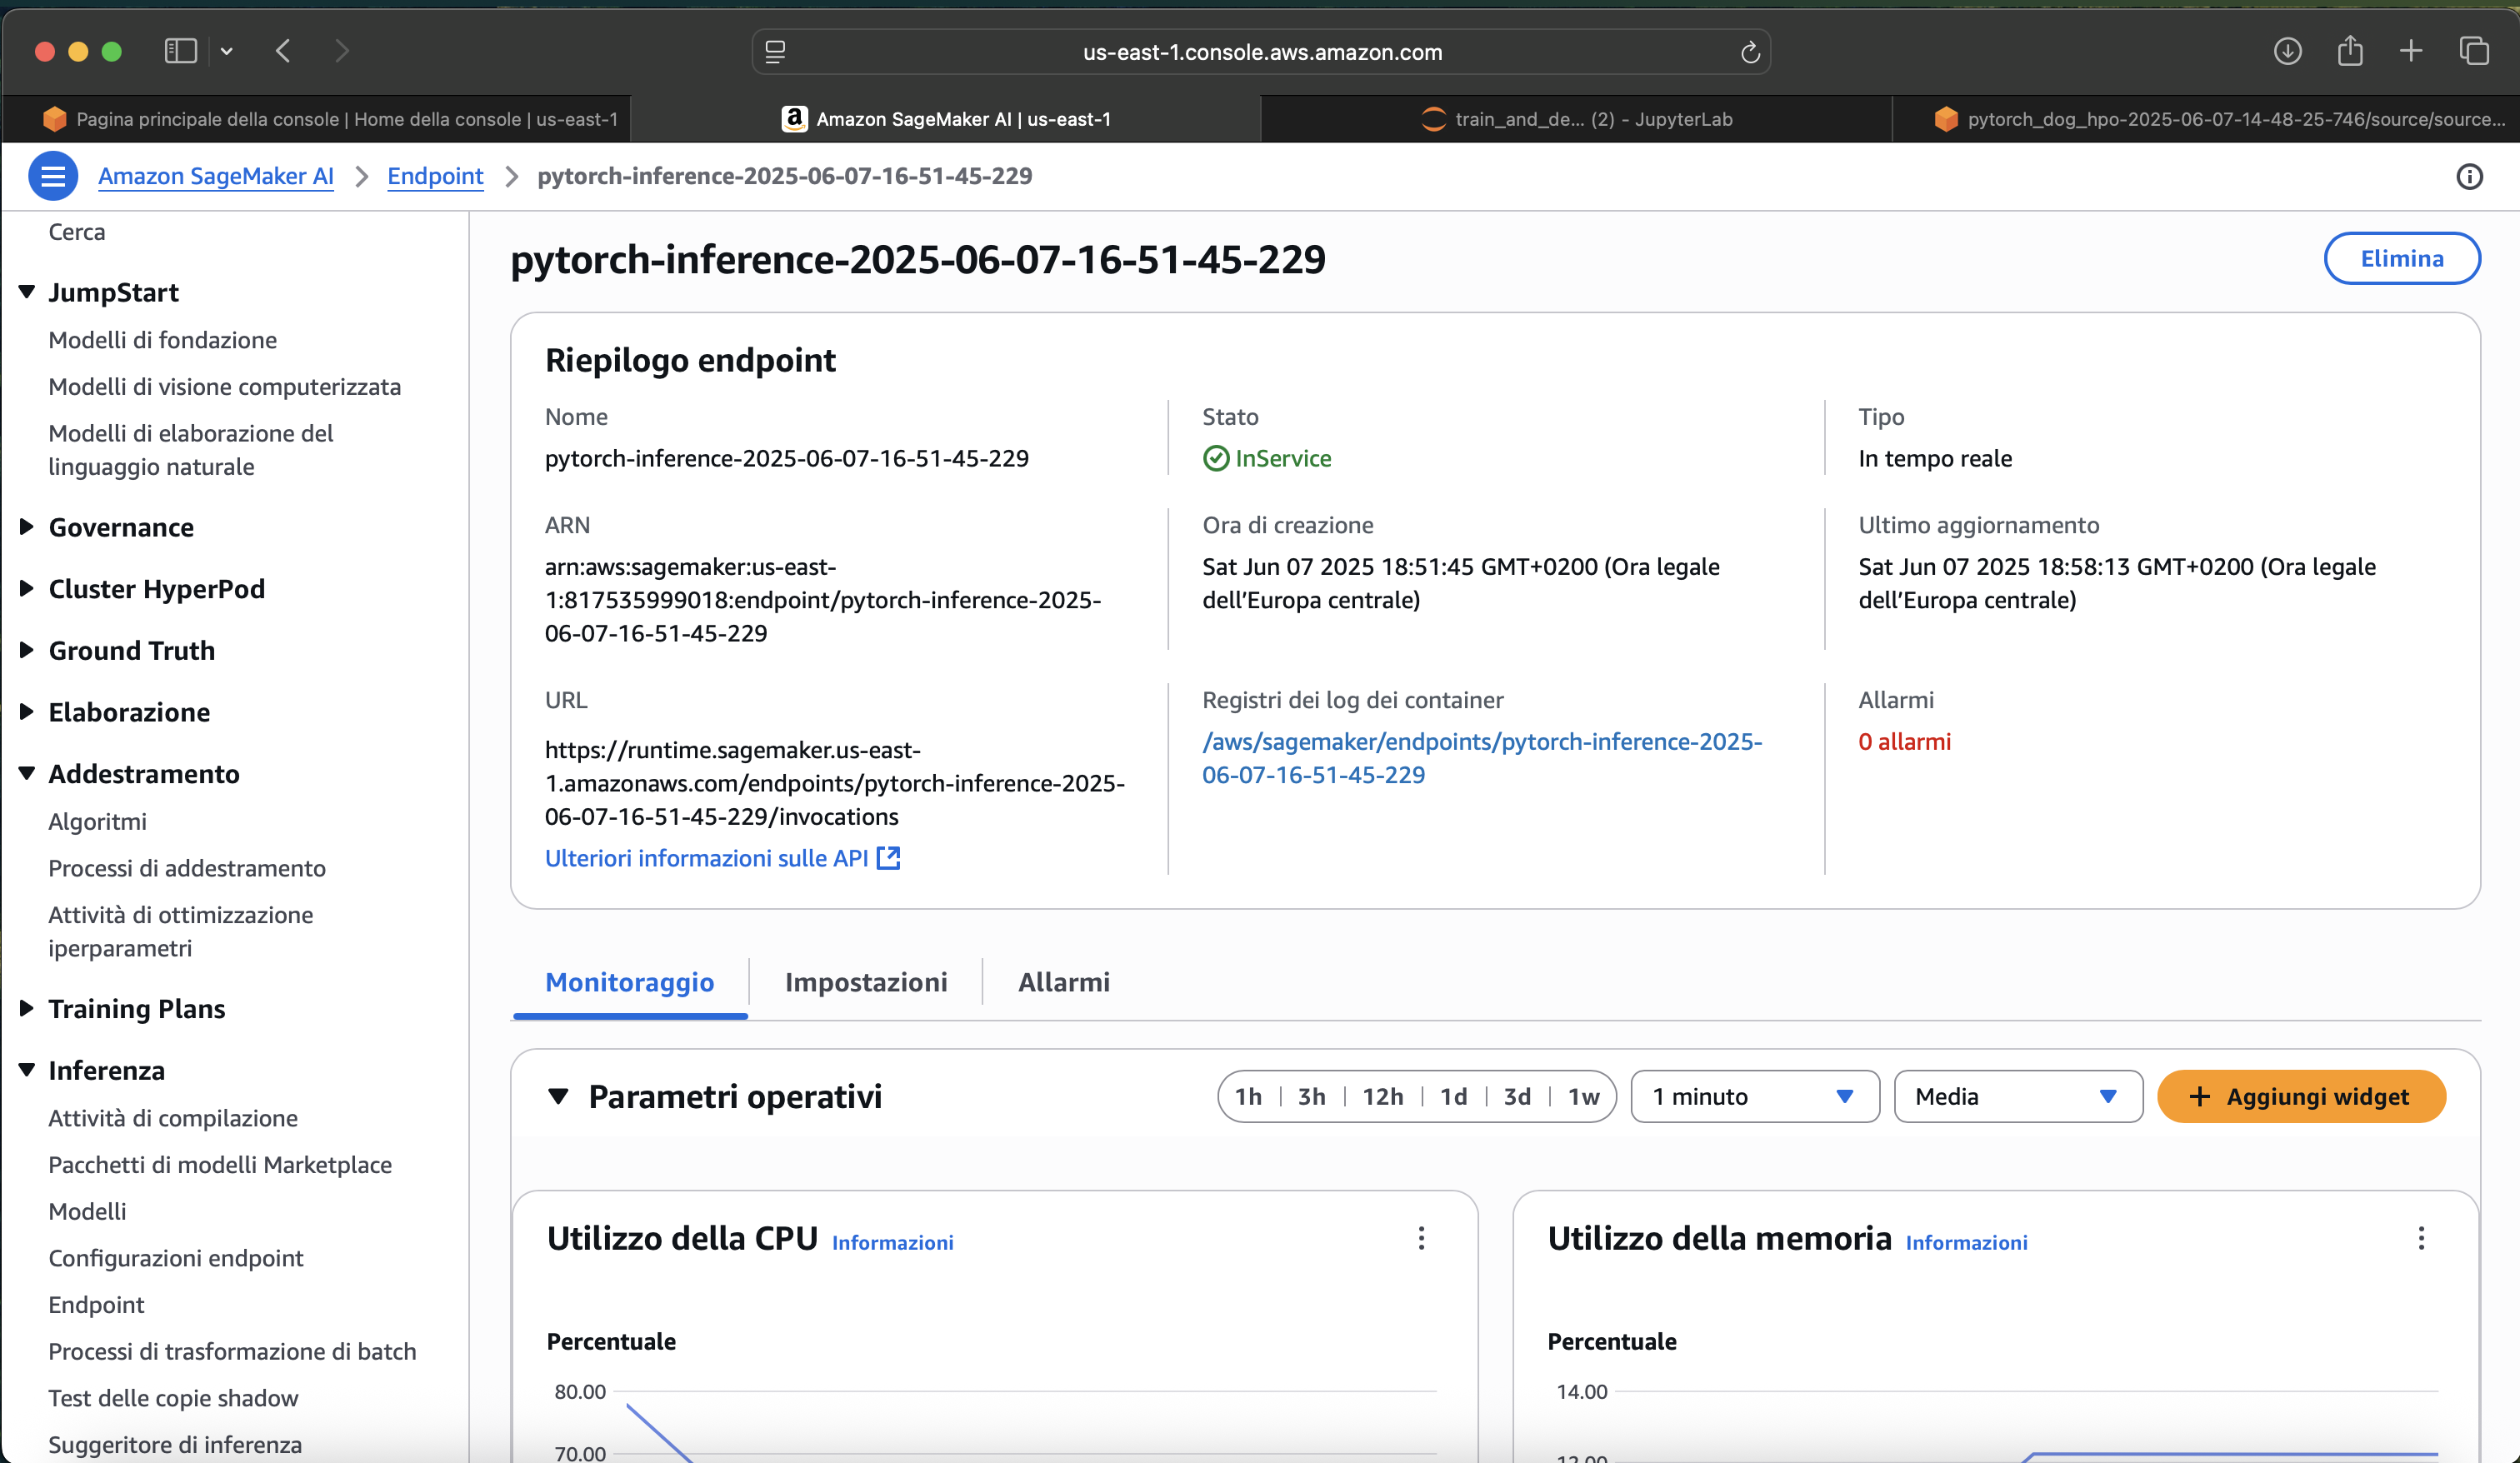
\includegraphics[width=0.7\textwidth]{img/Screenshot 2025-06-07 alle 19.00.39.png}
  \caption{screenshot showing a created Endpoint for the multy instance.}
  \label{fig:example}
\end{figure}

\section{Step 2: EC2 Training}
For this section i run an EC2 with training image: 
\begin{verbatim}amazon/Deep Learning AMI Neuron (Amazon Linux 2023) 20250520\end{verbatim} using an m5.2xlarge because it is a good tradeoff between the task that i have to accomplish and the costs. 

\begin{figure}[htbp]
  \centering
  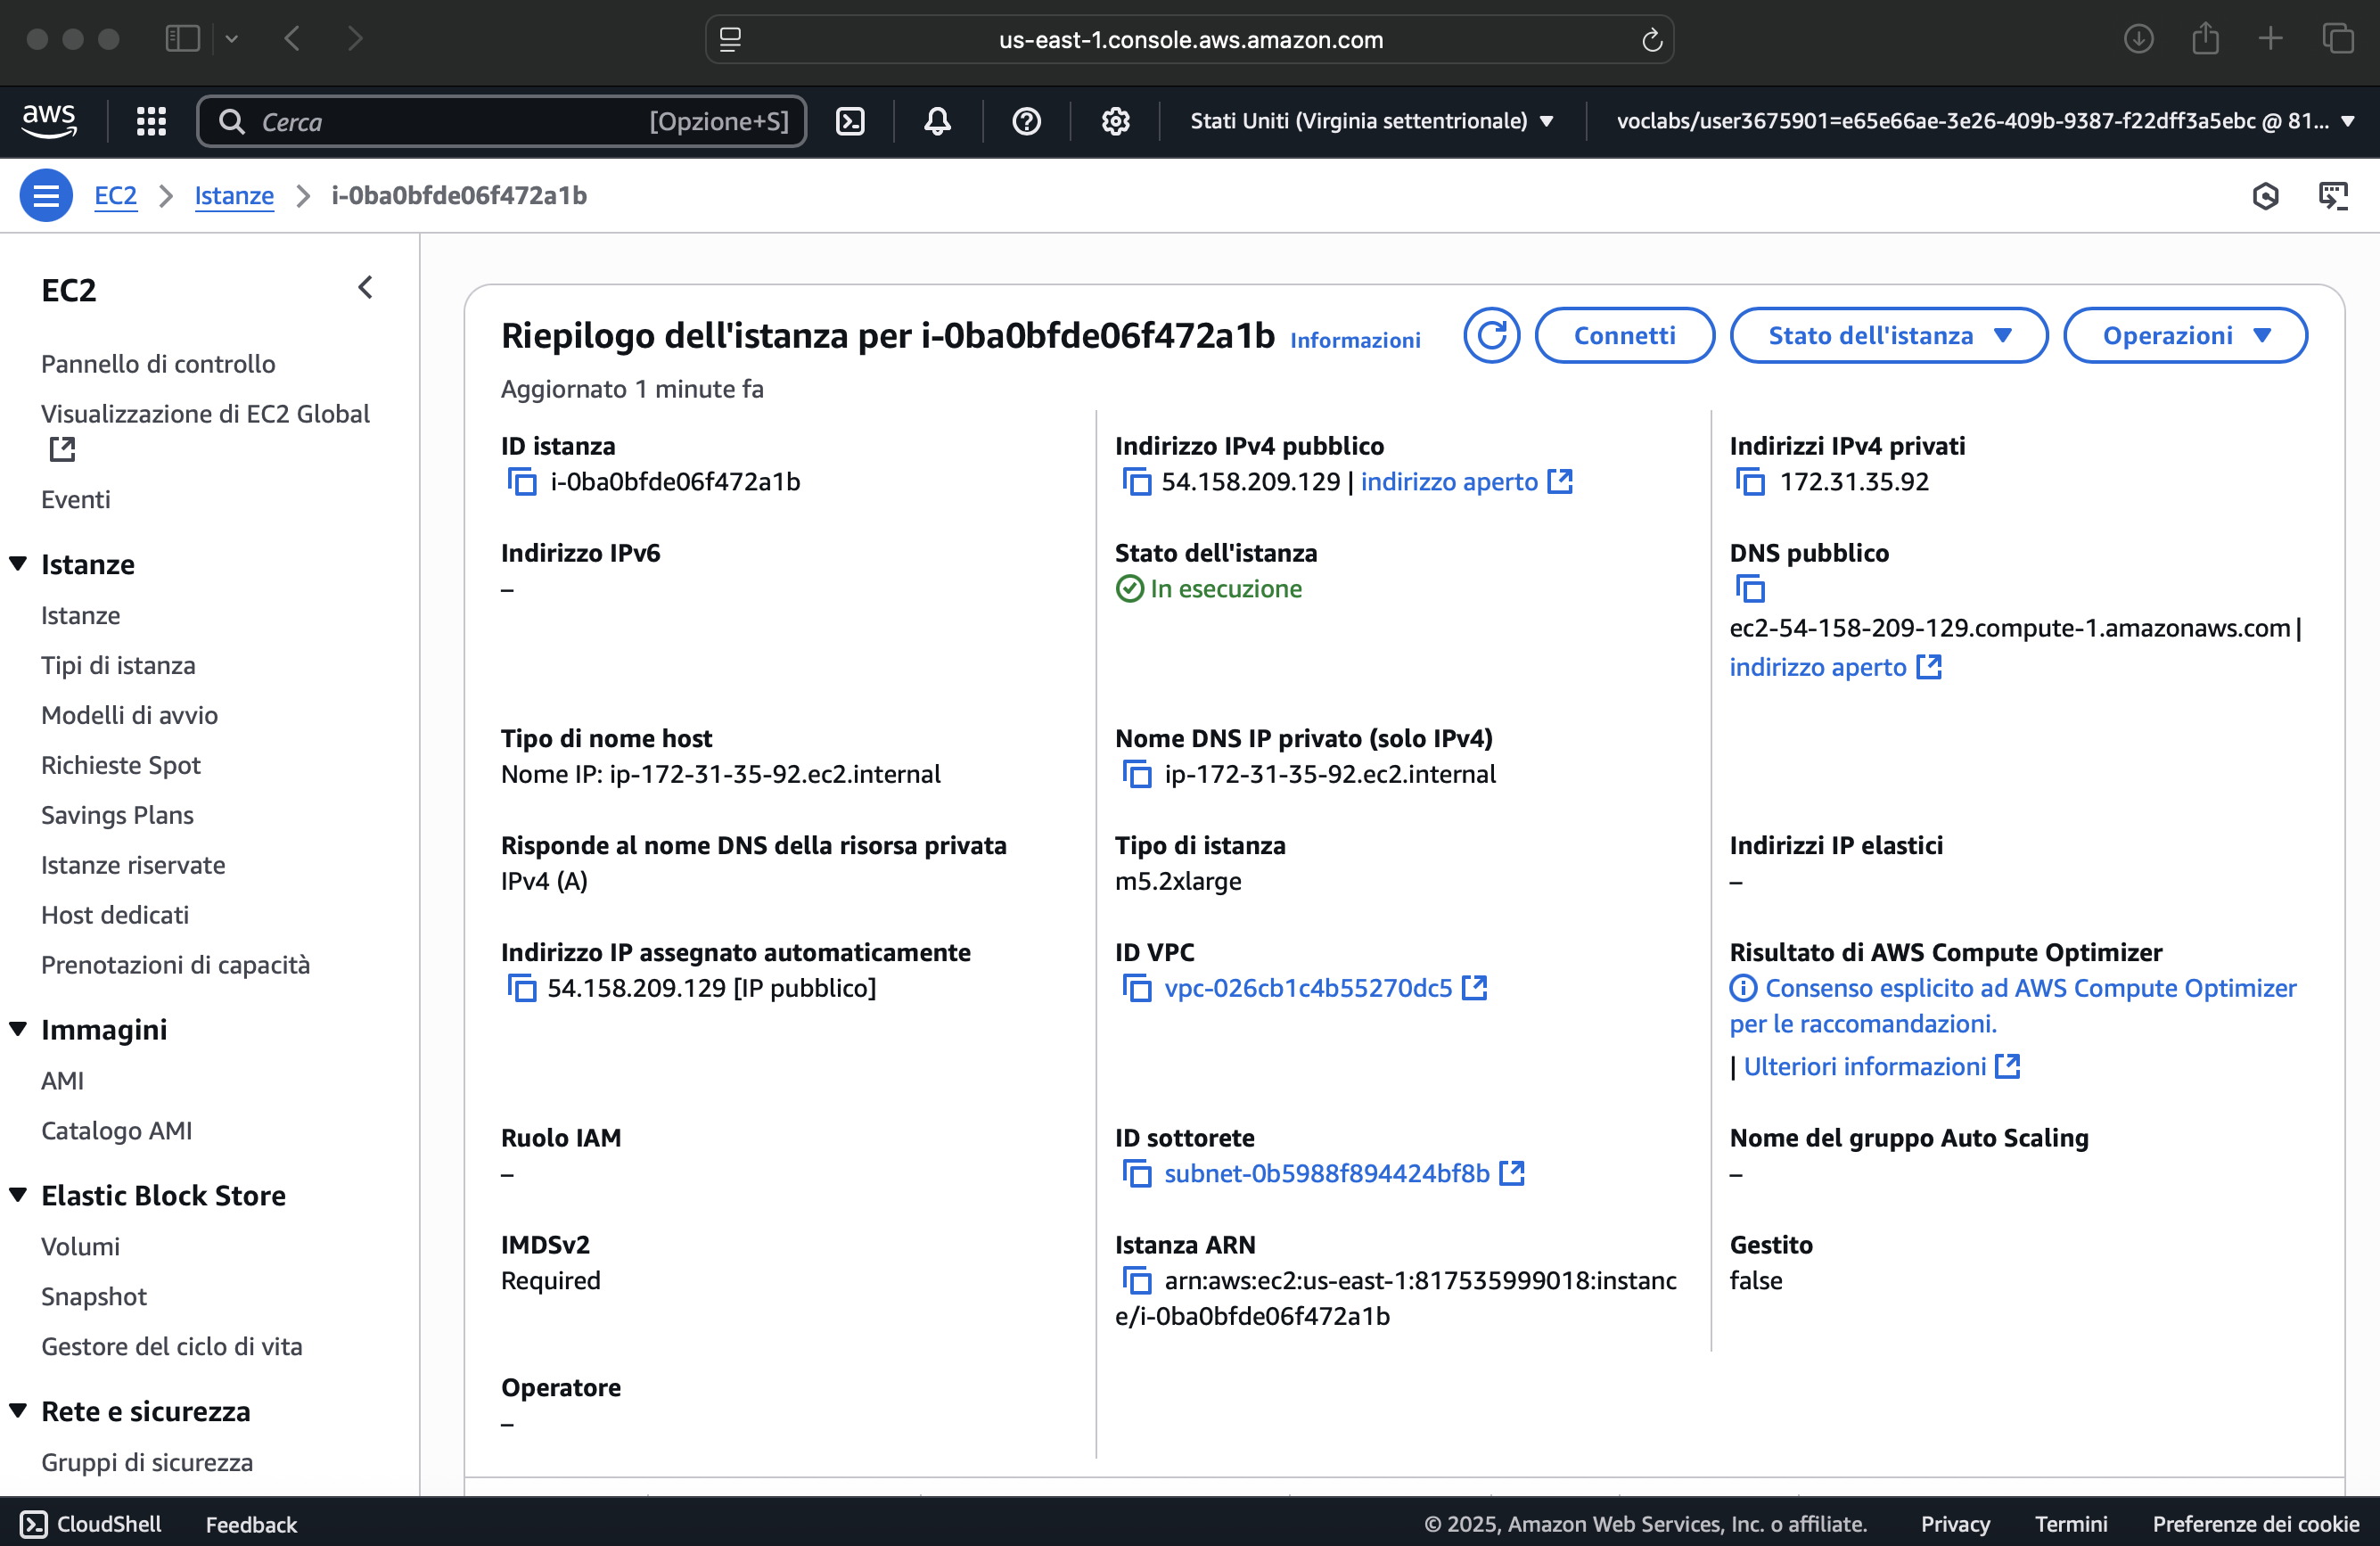
\includegraphics[width=0.7\textwidth]{img/Screenshot 2025-06-15 alle 14.49.34.png}
  \caption{screenshot showing a created EC2.}
  \label{fig:example}
\end{figure}

So I started it with the WAS UI and connected it with an SSH:
\begin{verbatim}ssh -i "ger.pem" ec2-user@ec2-54-158-209-129.compute-1.amazonaws.com\end{verbatim}

Once we are connected to our own EC2 we have to do the following step to: Download your own data, Create the target folder for the trained model, so we can copy the code for the train in a file called \textit{solution.py} and run it.  

\begin{verbatim}
wget https://s3-us-west-1.amazonaws.com/udacity-aind/dog project/dogImages.zip
unzip dogImages.zip
mkdir TrainedModel 
nano solution.py
python solution.py
\end{verbatim}

\begin{figure}[htbp]
  \centering
  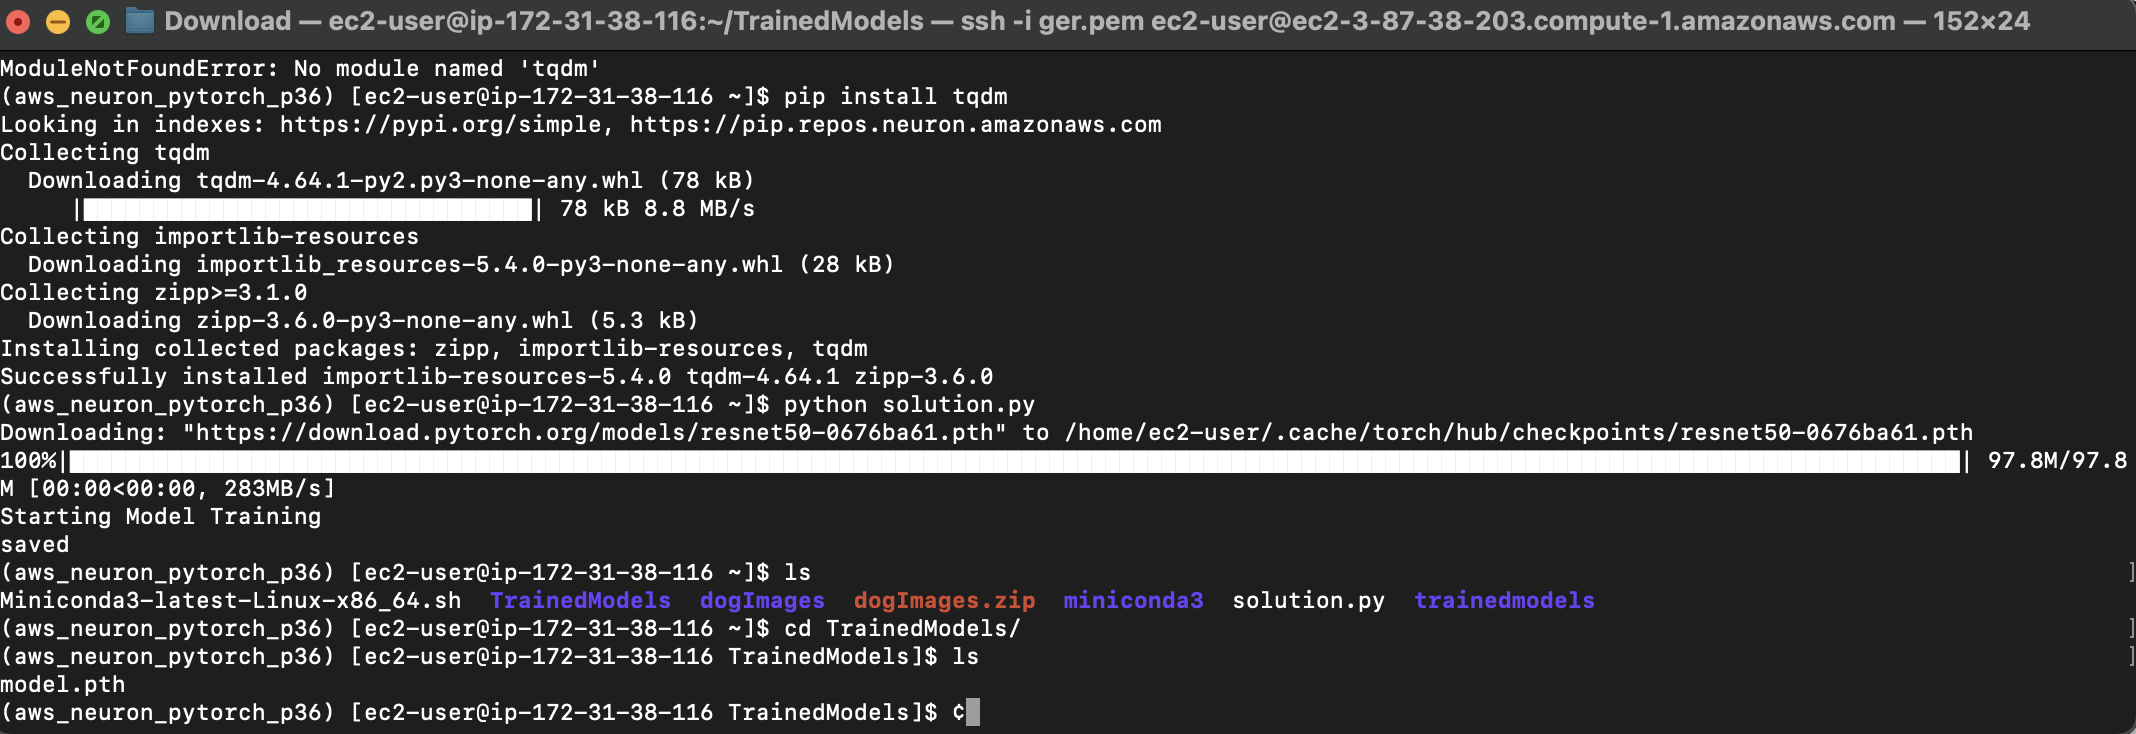
\includegraphics[width=0.7\textwidth]{img/Screenshot 2025-06-15 alle 16.09.31.png}
  \caption{screenshot showing a finished training model.}
  \label{fig:example}
\end{figure}

I found some problem with the env that i had to create and install different missing pips.

\subsection{Differances between the Sagemaker Notebook and EC2}
In the Sagemaker we create a Nootebook instance where we write the code to create and instance to perform the training but in the EC2 we directly run the script code "localy" in the EC2.
\begin{itemize}
  \item In the Sagemaker the hyperparameters are passed to hpo.py as an argument, but in the EC2 we run directly the hpo in the script.
  \item Using the EC2 we limited just to this instance but if we used the Sagemaker Notenook we can used the coded seen befored to perform distribuited trainig
  \item The final model, in the EC2 we have the model saved in then target folder, if we would like to save it in the could we should run the code wo upload it in the S3 bucket but using the Sagemaker Nootebook the "artifact" with is the model and the hpo are directly saved in a S3 target foolder.
\end{itemize}

\section{Step 3: Lambda Fuction}
So the Lambda function created takes the endpoint created in the previous steps and makes inferences passing the S3 url of it. So in this i passed the name of my endpoint to my lambda function: \textit{ pytorch-inference-2025-06-15-15-57-32-476}. 

\section{Step 4: Lambda Security and Testing}

Now i sended to the Endpoint this image path to do an inference: 
\begin{verbatim}https://s3.amazonaws.com/cdn-origin-etr.akc.org/wp-content/uploads/2017/11/20113314/Carolina-Dog-standing-outdoors.jpg"\end{verbatim}
Which is the same one used to do inference in the previous steps, for the security consideration i created a restricted policy to have just the specific Endpoint Access so this LambdaFuction can't perform other action to my other Endpoints.

\begin{figure}[htbp]
  \centering
  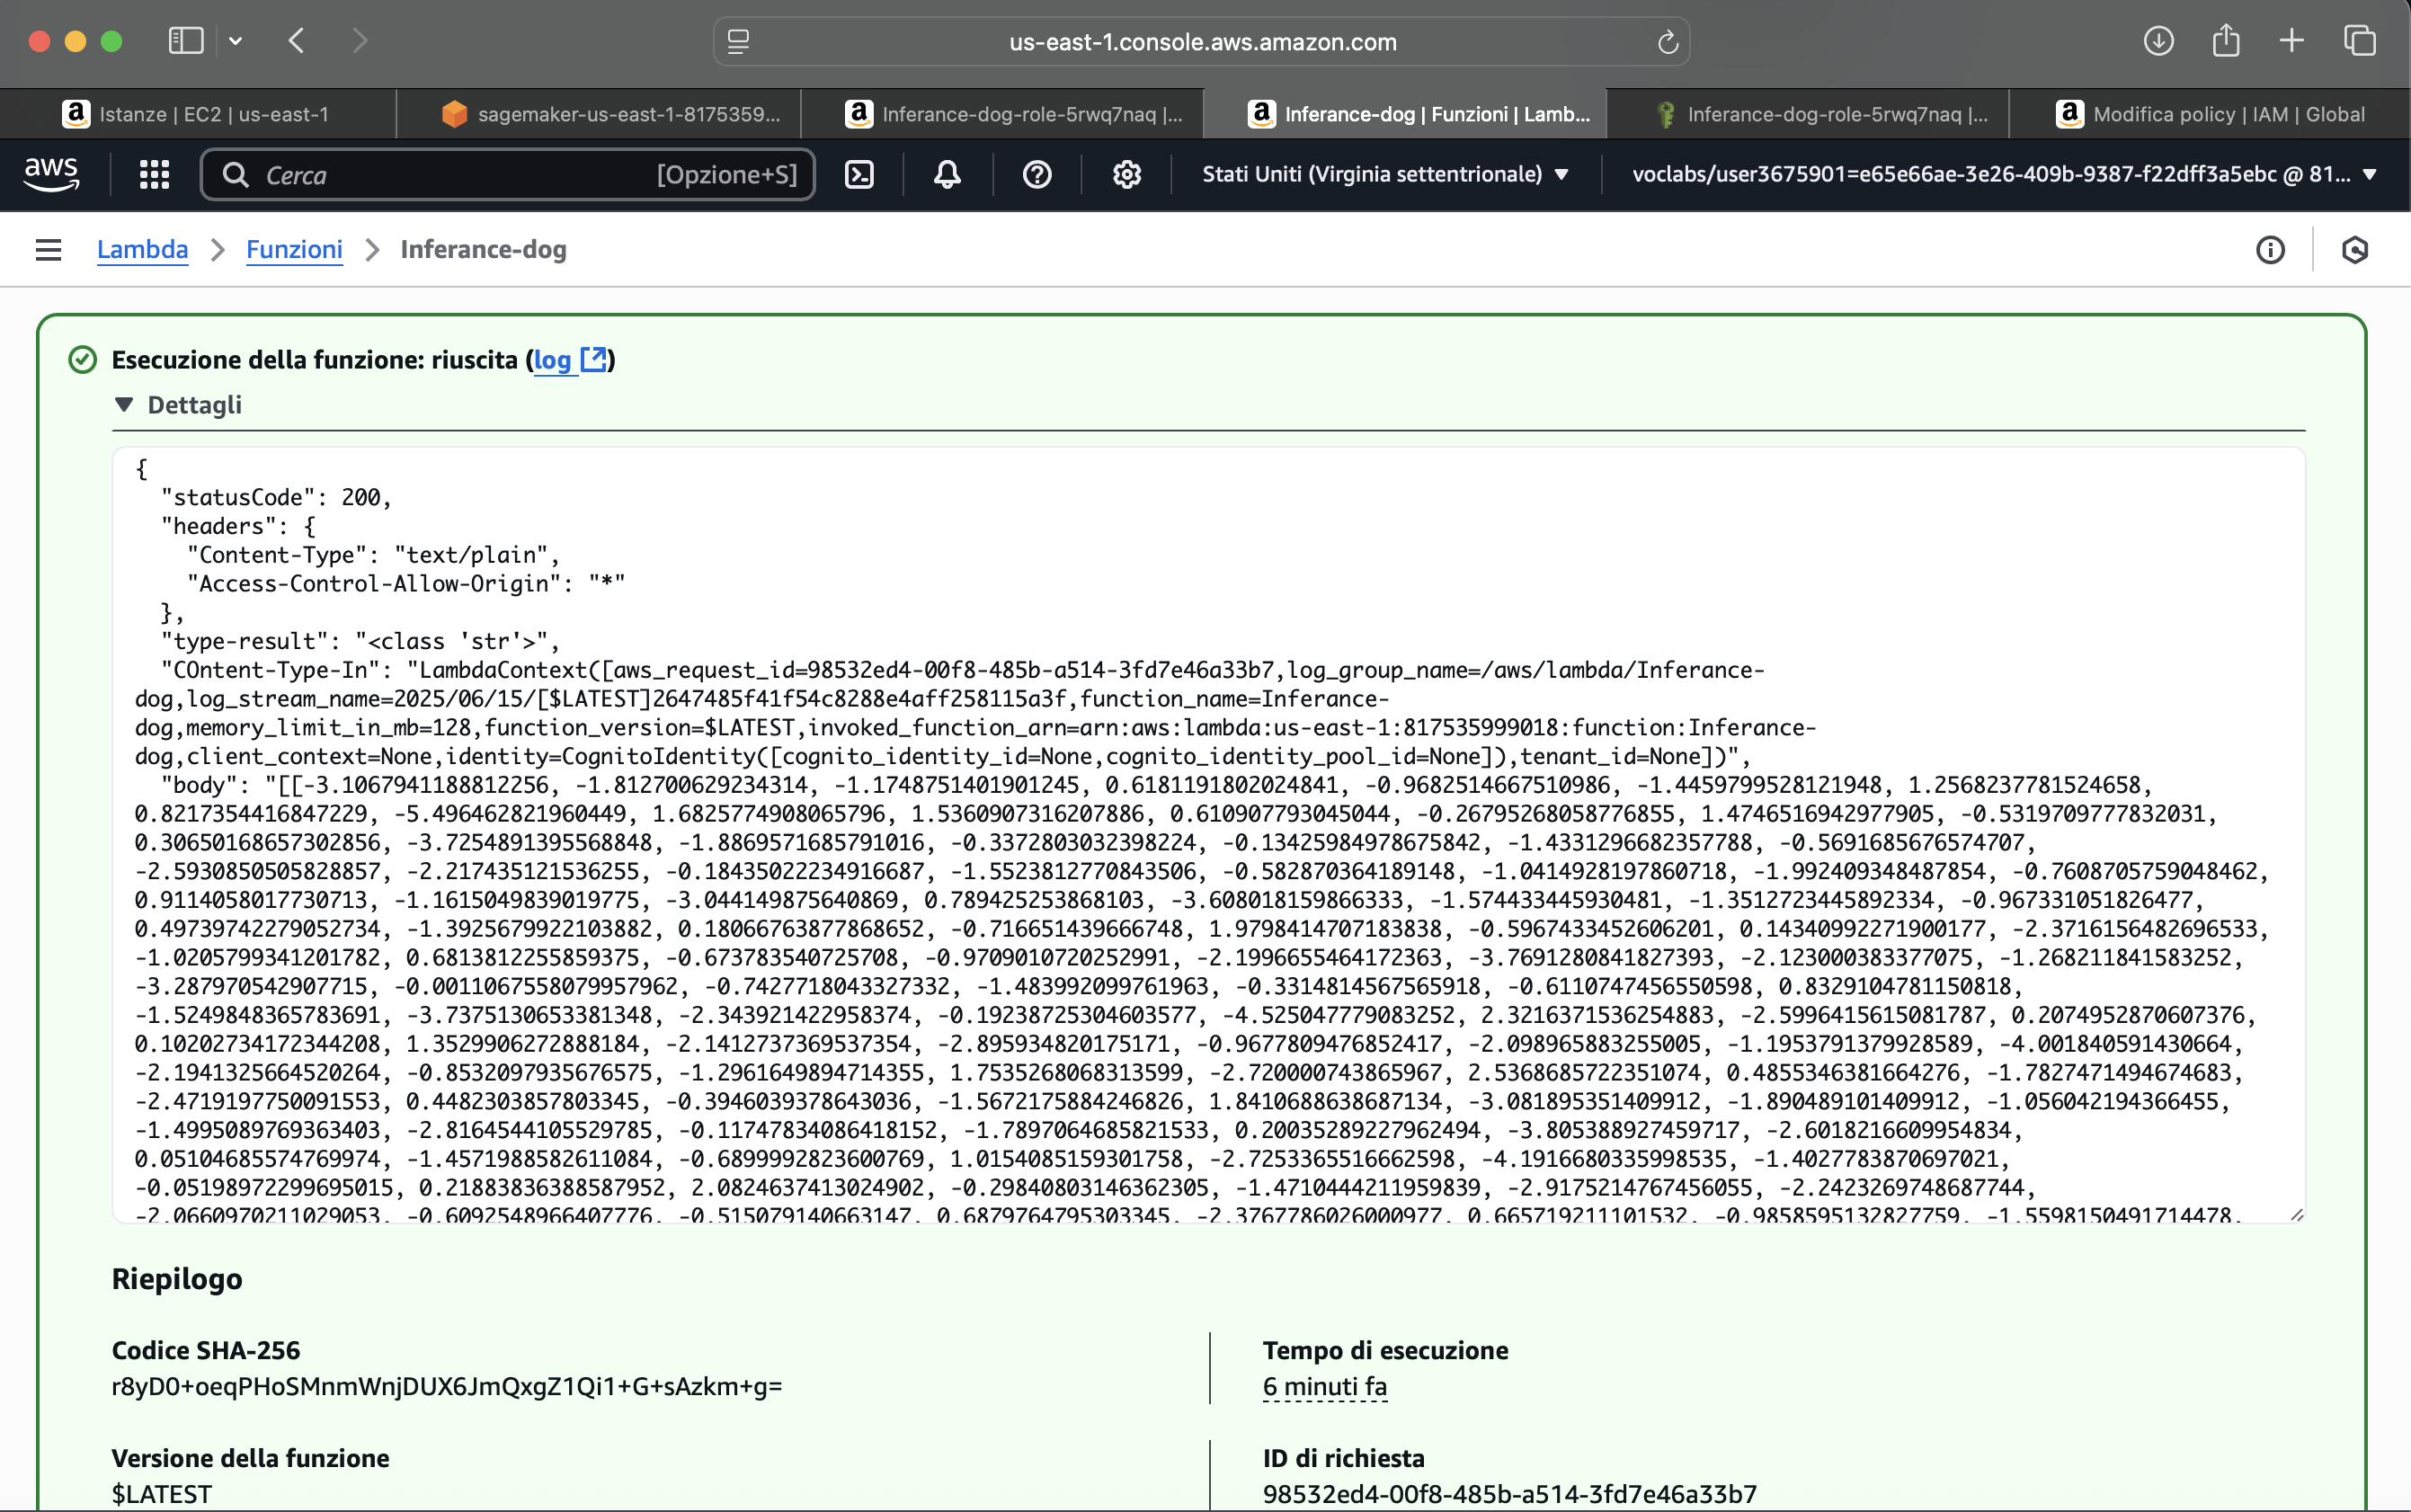
\includegraphics[width=0.7\textwidth]{img/Screenshot 2025-06-15 alle 18.27.44.png}
  \caption{screenshot showing a inference made with my LambdaFuction.}
  \label{fig:example}
\end{figure}

\newpage

\begin{figure}[htbp]
  \centering
  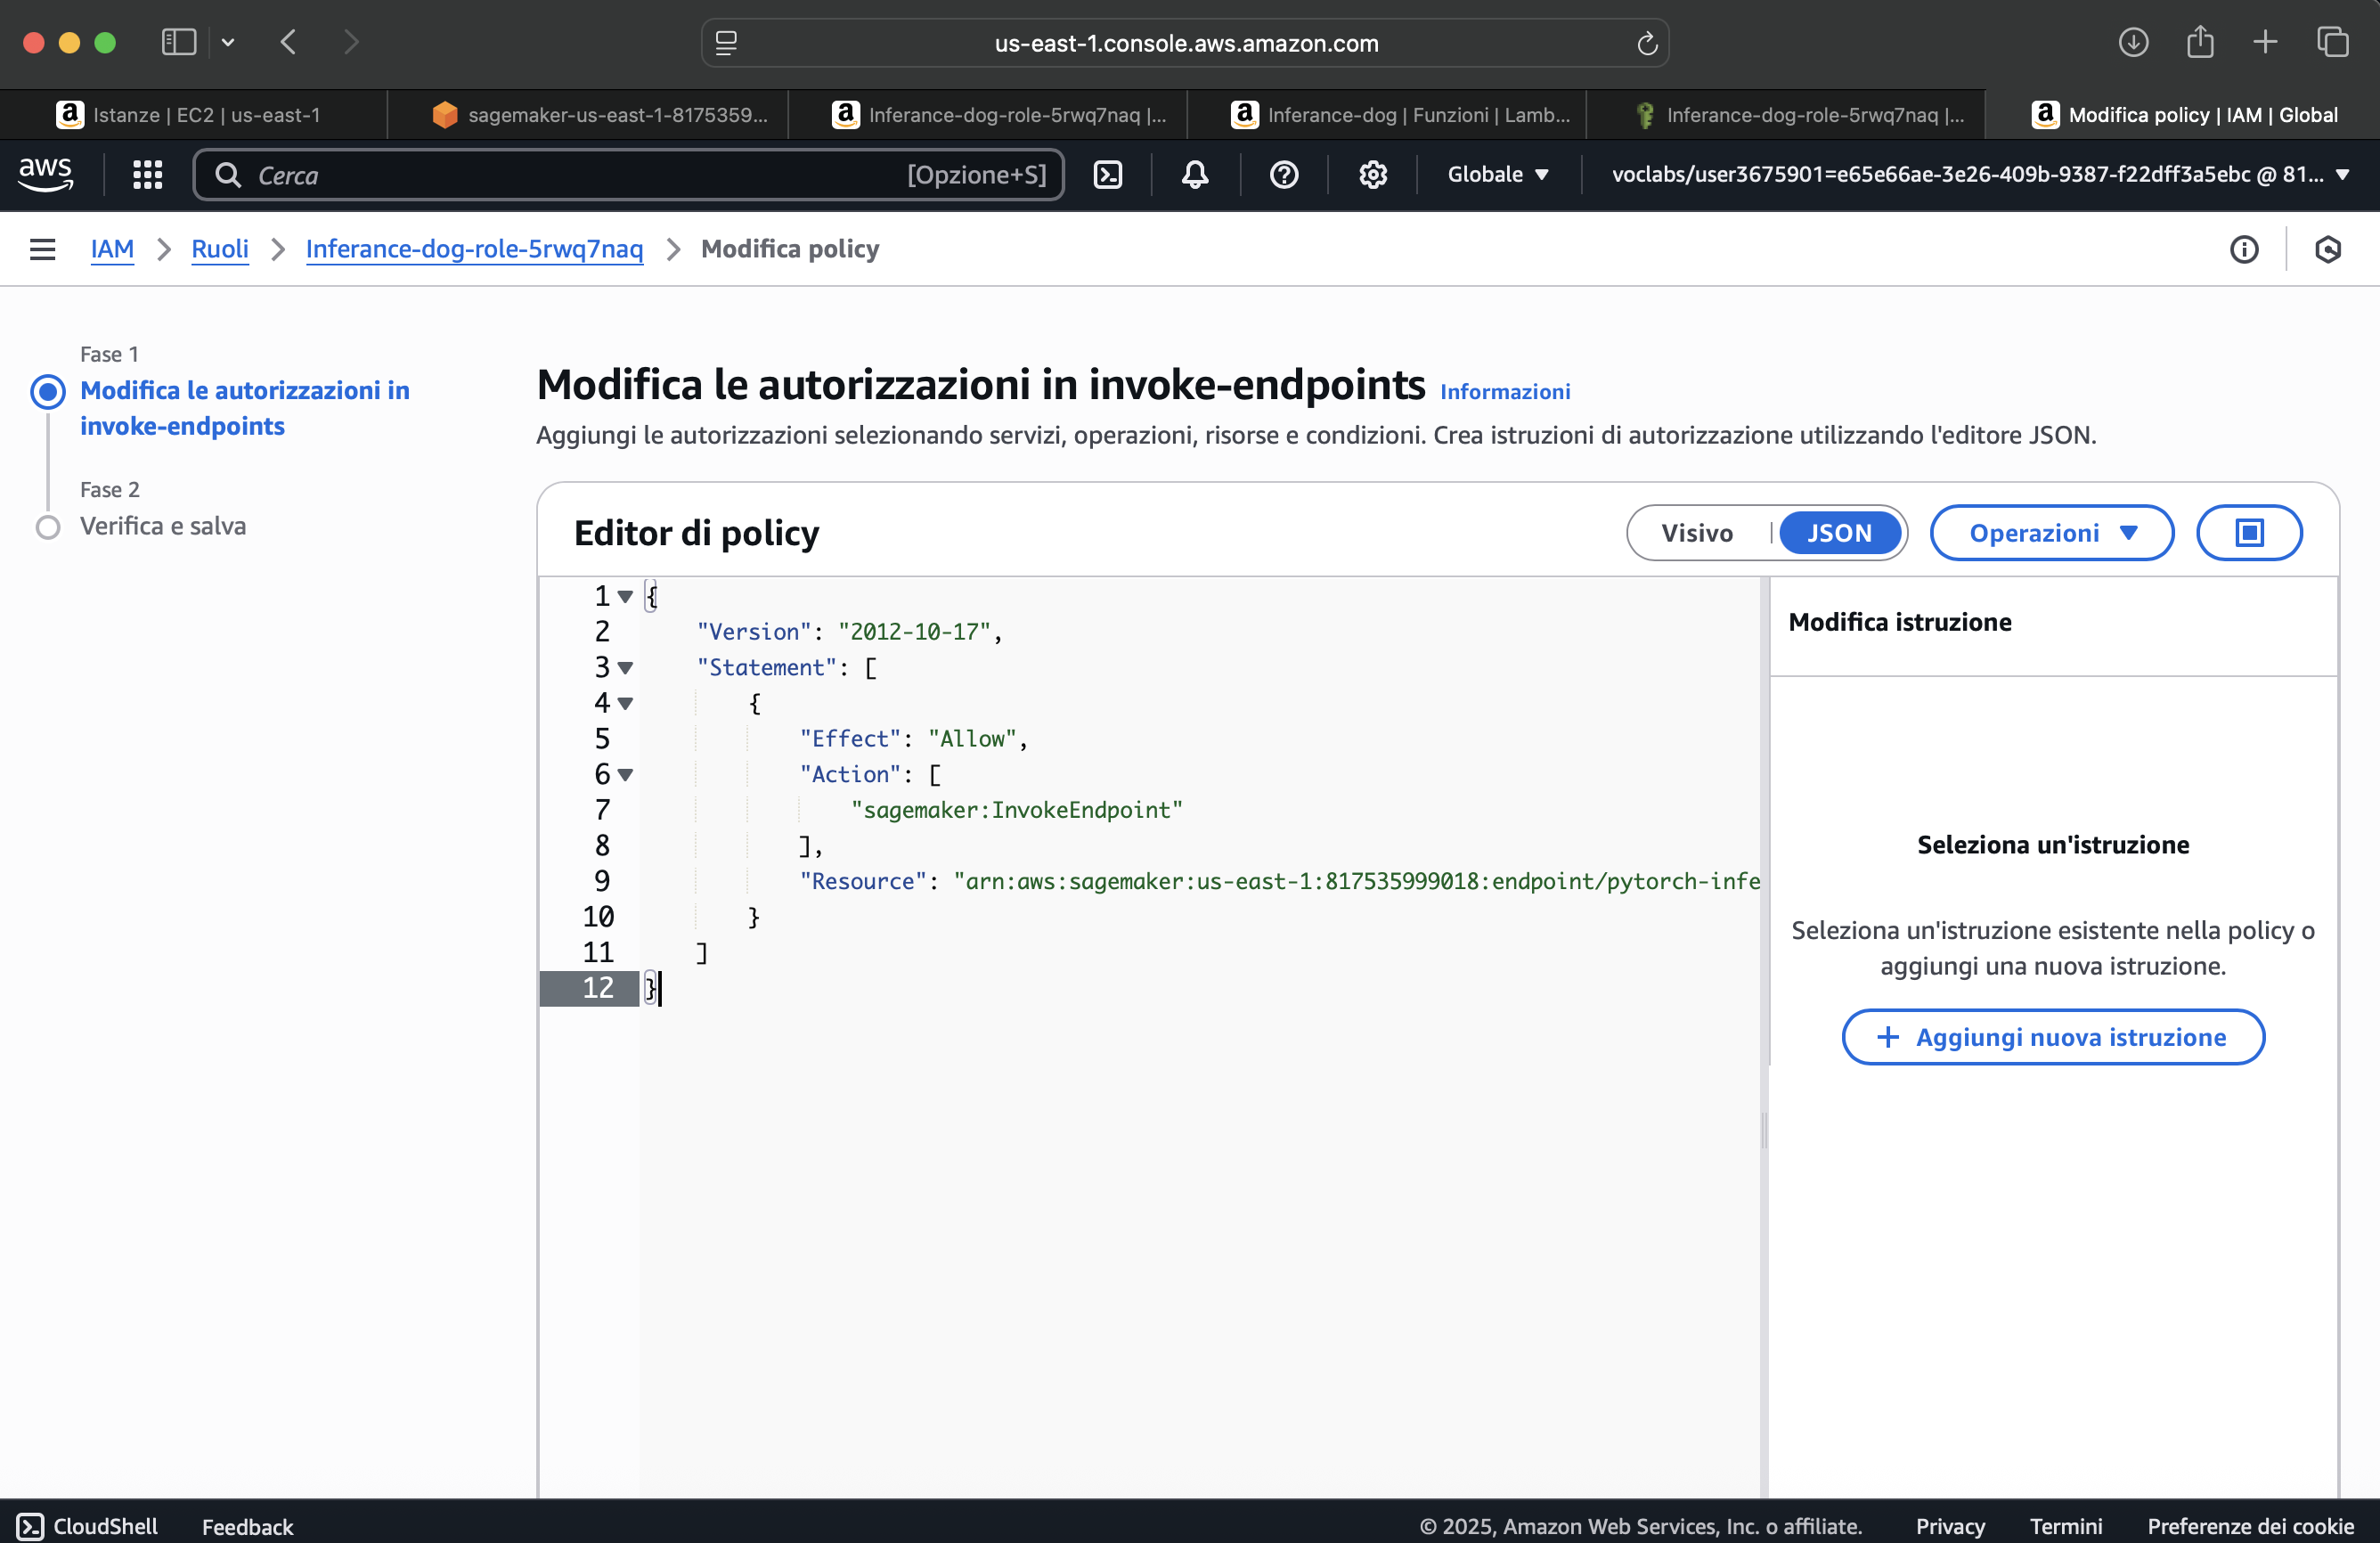
\includegraphics[width=0.7\textwidth]{img/Screenshot 2025-06-15 alle 18.27.03.png}
  \caption{screenshot showing the specific policy for my LambdaFunction.}
  \label{fig:example}
\end{figure}

% Add as many sections as needed

\section{Step 5: Concurrency and Auto-Scaling}
\subsection{Concurrency}
Concurrency refers to the ability of Lambda functions to handle multiple requests simultaneously.

We can configure either Reserved or Provisioned concurrency for our function. Provisioned concurrency provides faster response times but comes with higher cost.

Because our expected request volume is low, we don’t need very high concurrency. I have set Provisioned concurrency to 3, which is sufficient for our needs, and Reserved concurrency to 100.

Below is a screenshot of the Lambda concurrency settings:

\begin{figure}[htbp]
  \centering
  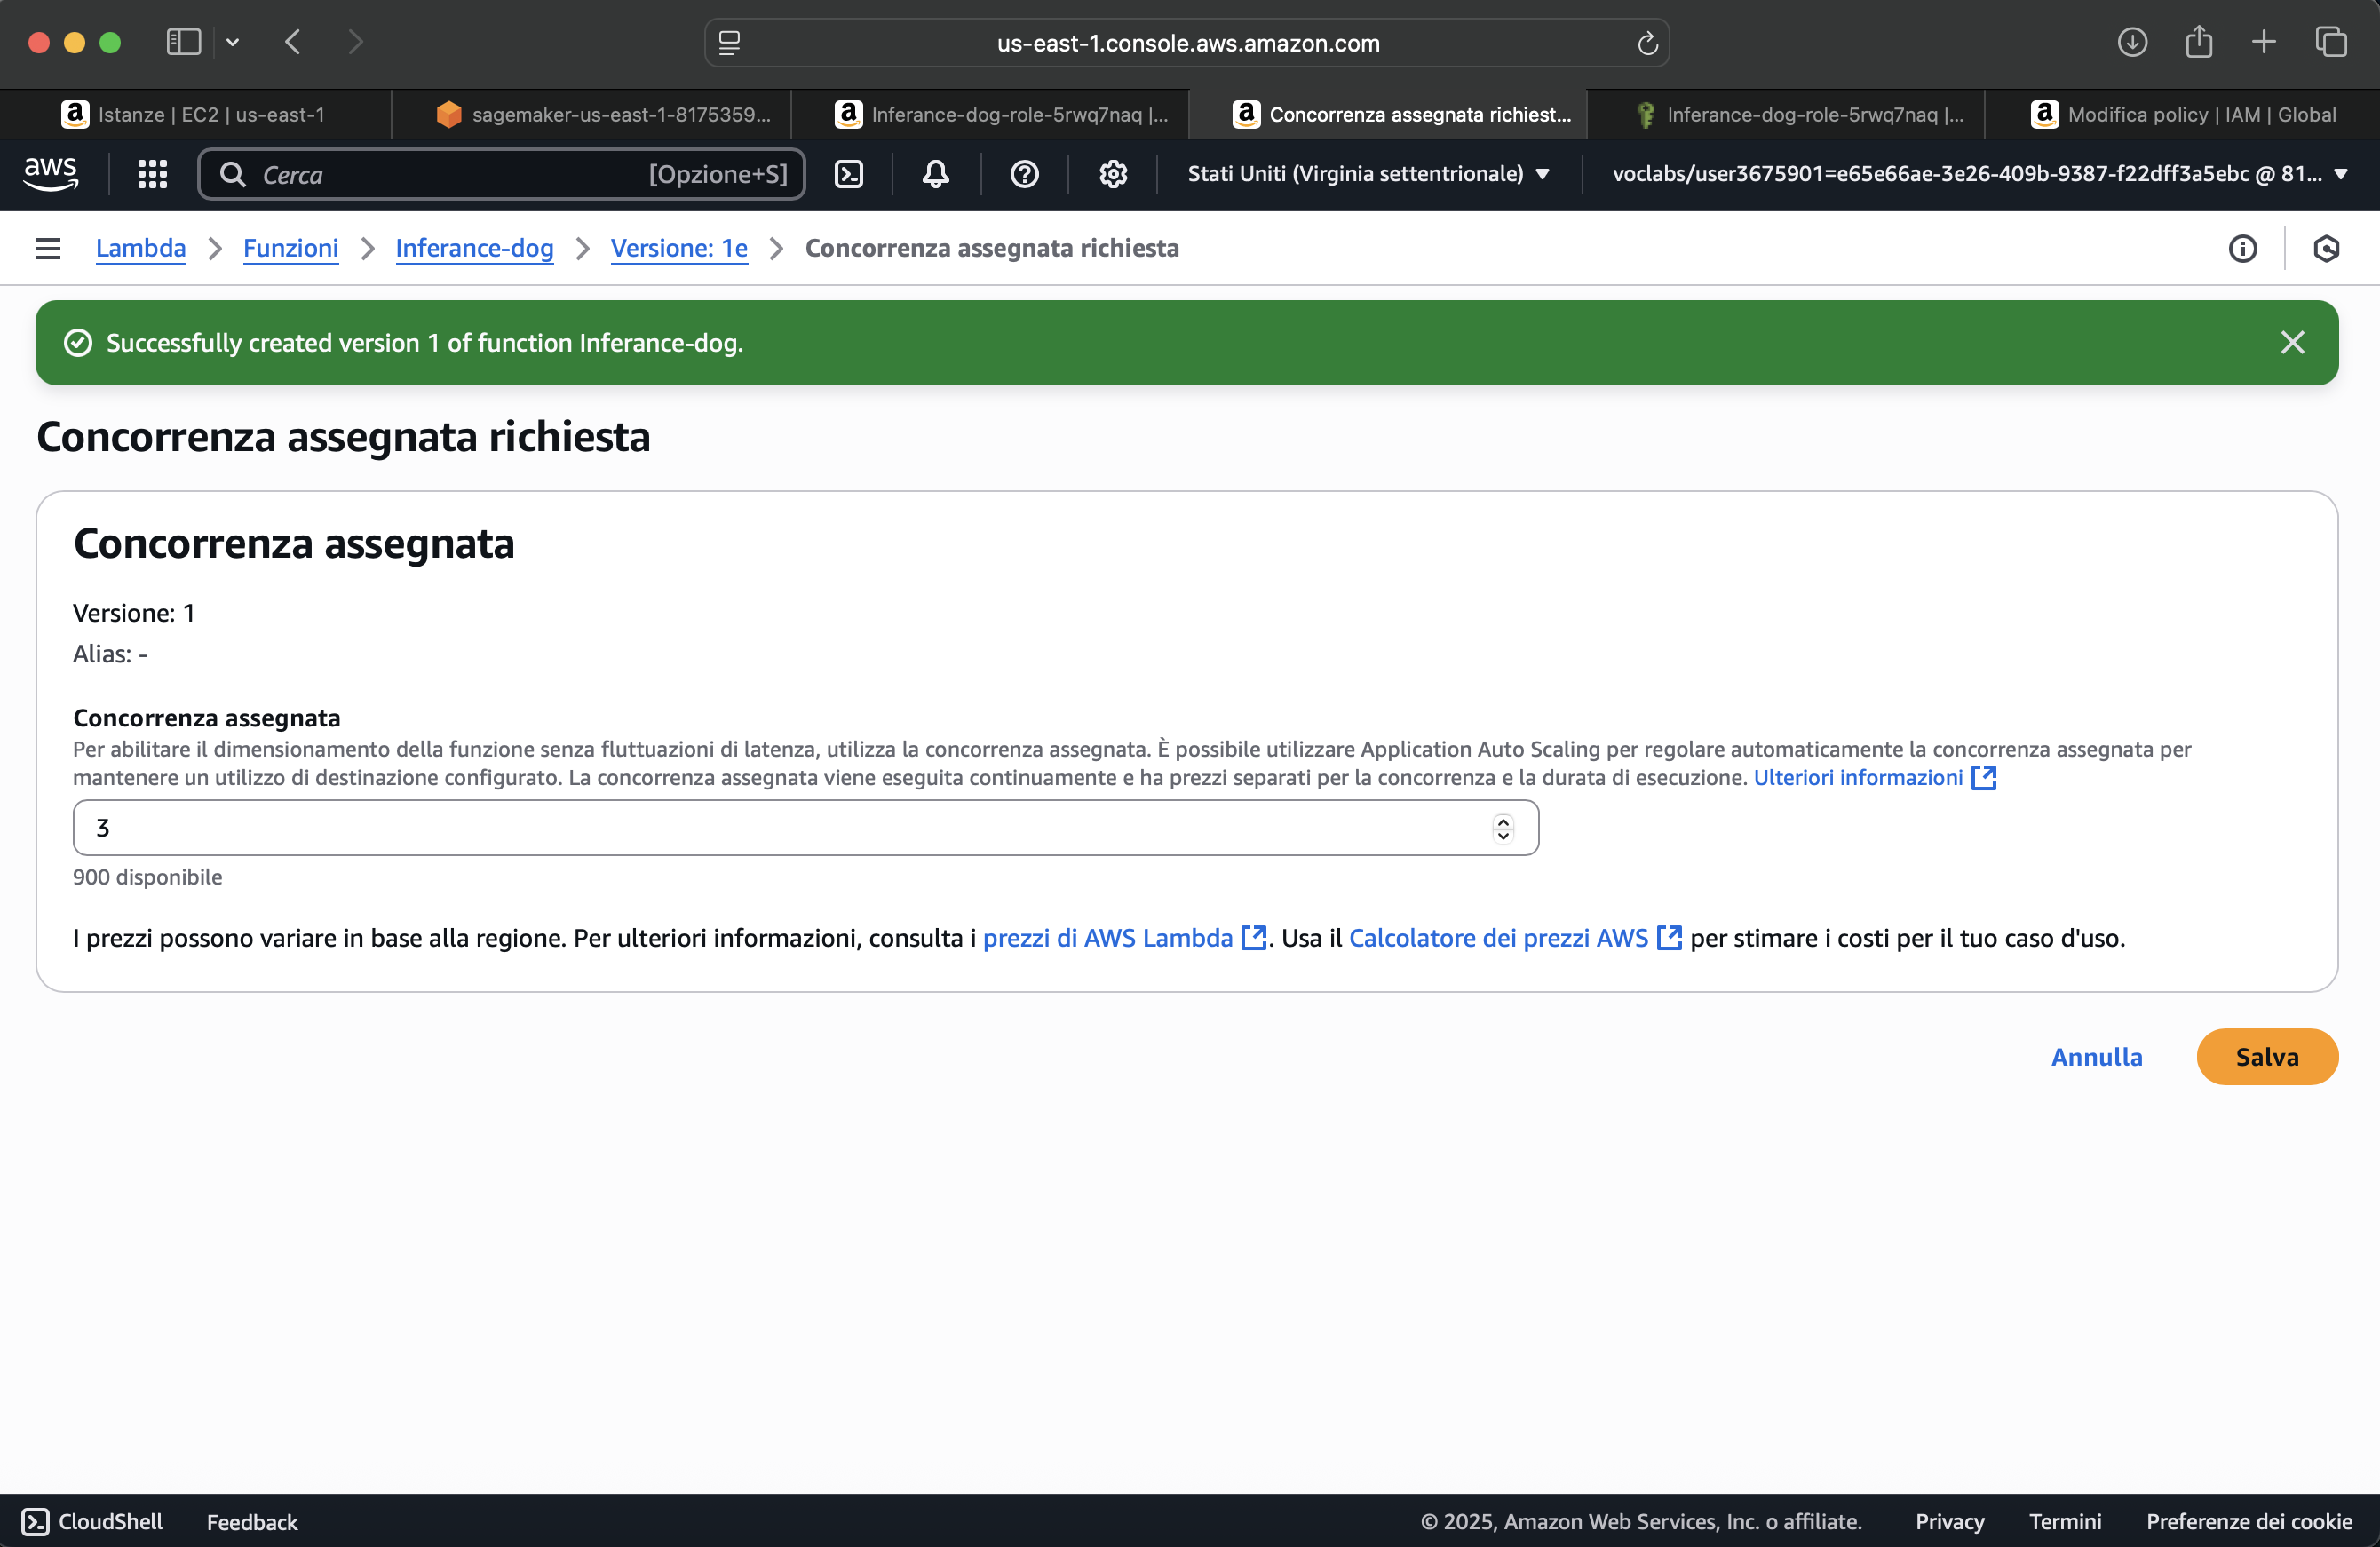
\includegraphics[width=0.7\textwidth]{img/Screenshot 2025-06-15 alle 18.51.31.png}
  \caption{screenshot showing the concurrency settins.}
  \label{fig:example}
\end{figure}

\subsection{Auto-scaling}
Auto-scaling refers to the ability of endpoints to service multiple
lambda function requests at once. I chose to autoscale endpoints to 4
instances maximum, with scale in coold down time of 30 seconds and scale
out cool down time of 300 seconds. These settings are sufficient for our
project needs and workload.

\end{document}